\section{Day 2: More Transistors and Circuit Creation (Sept 9, 2025)}

The goal of today is to understand what's inside a gate, and for us to never think about the underlying transistors going on inside ever again. We wish to abstract away such details, and aim for more modular designs. 

\subsection{Transistors}

\begin{problem}
Why is NAND the most common gate?
\end{problem}

\textbf{nMOS} transistors has its source and drain connected when the input (gate voltage) is high, and \textbf{pMOS} transistors connect when the input is low.

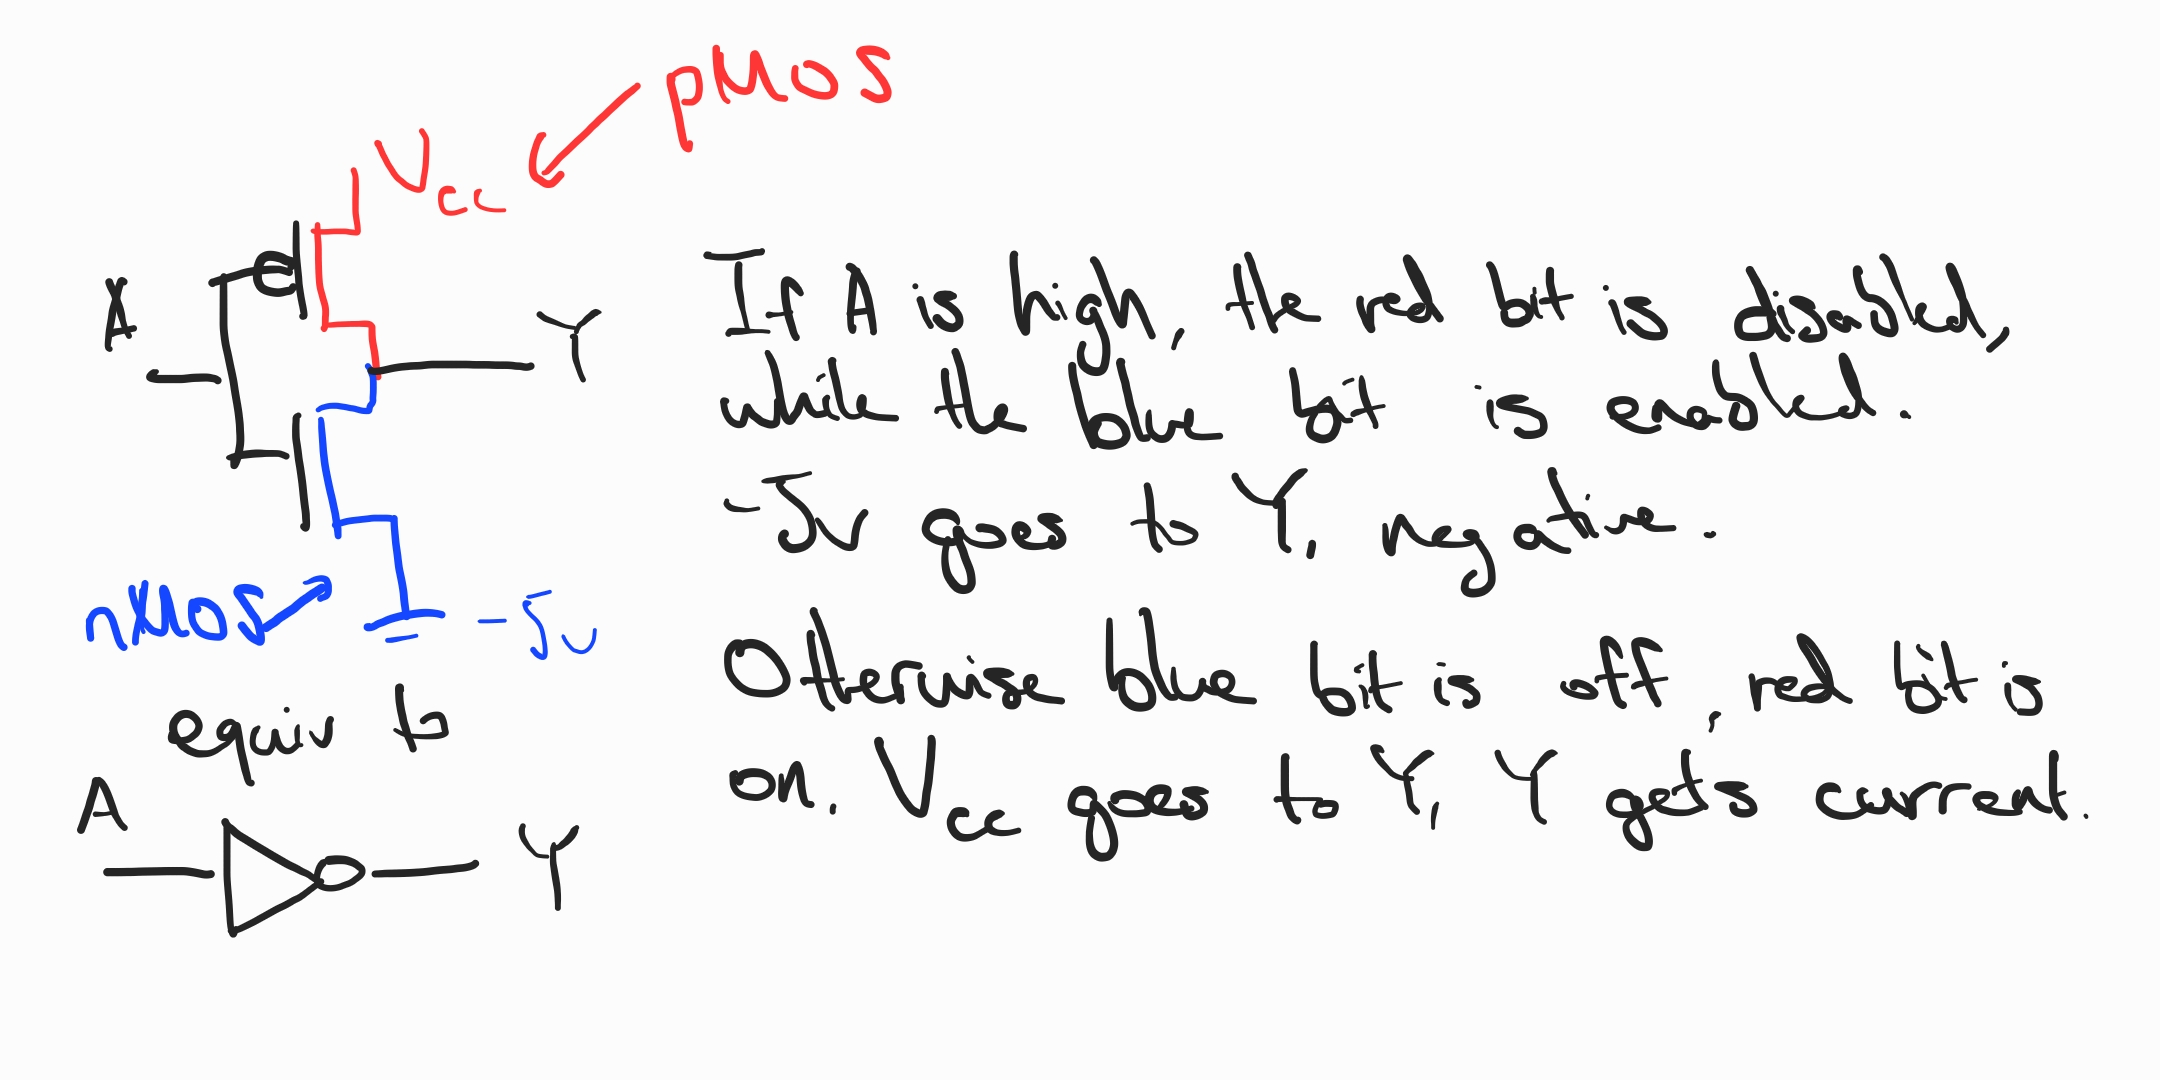
\includegraphics{csc258/figures/nmospmosnotgate.jpg}

$V_{cc}$ is ``common collector voltage'' which is high voltage ($5V$) in this course. You need to \textit{explicitly} connect the output to one of $V_{cc}$ and ground for it to be high and low respectively. Otherwise, the result could be high or low. This is what an AND gate looks like at the transistor-level:

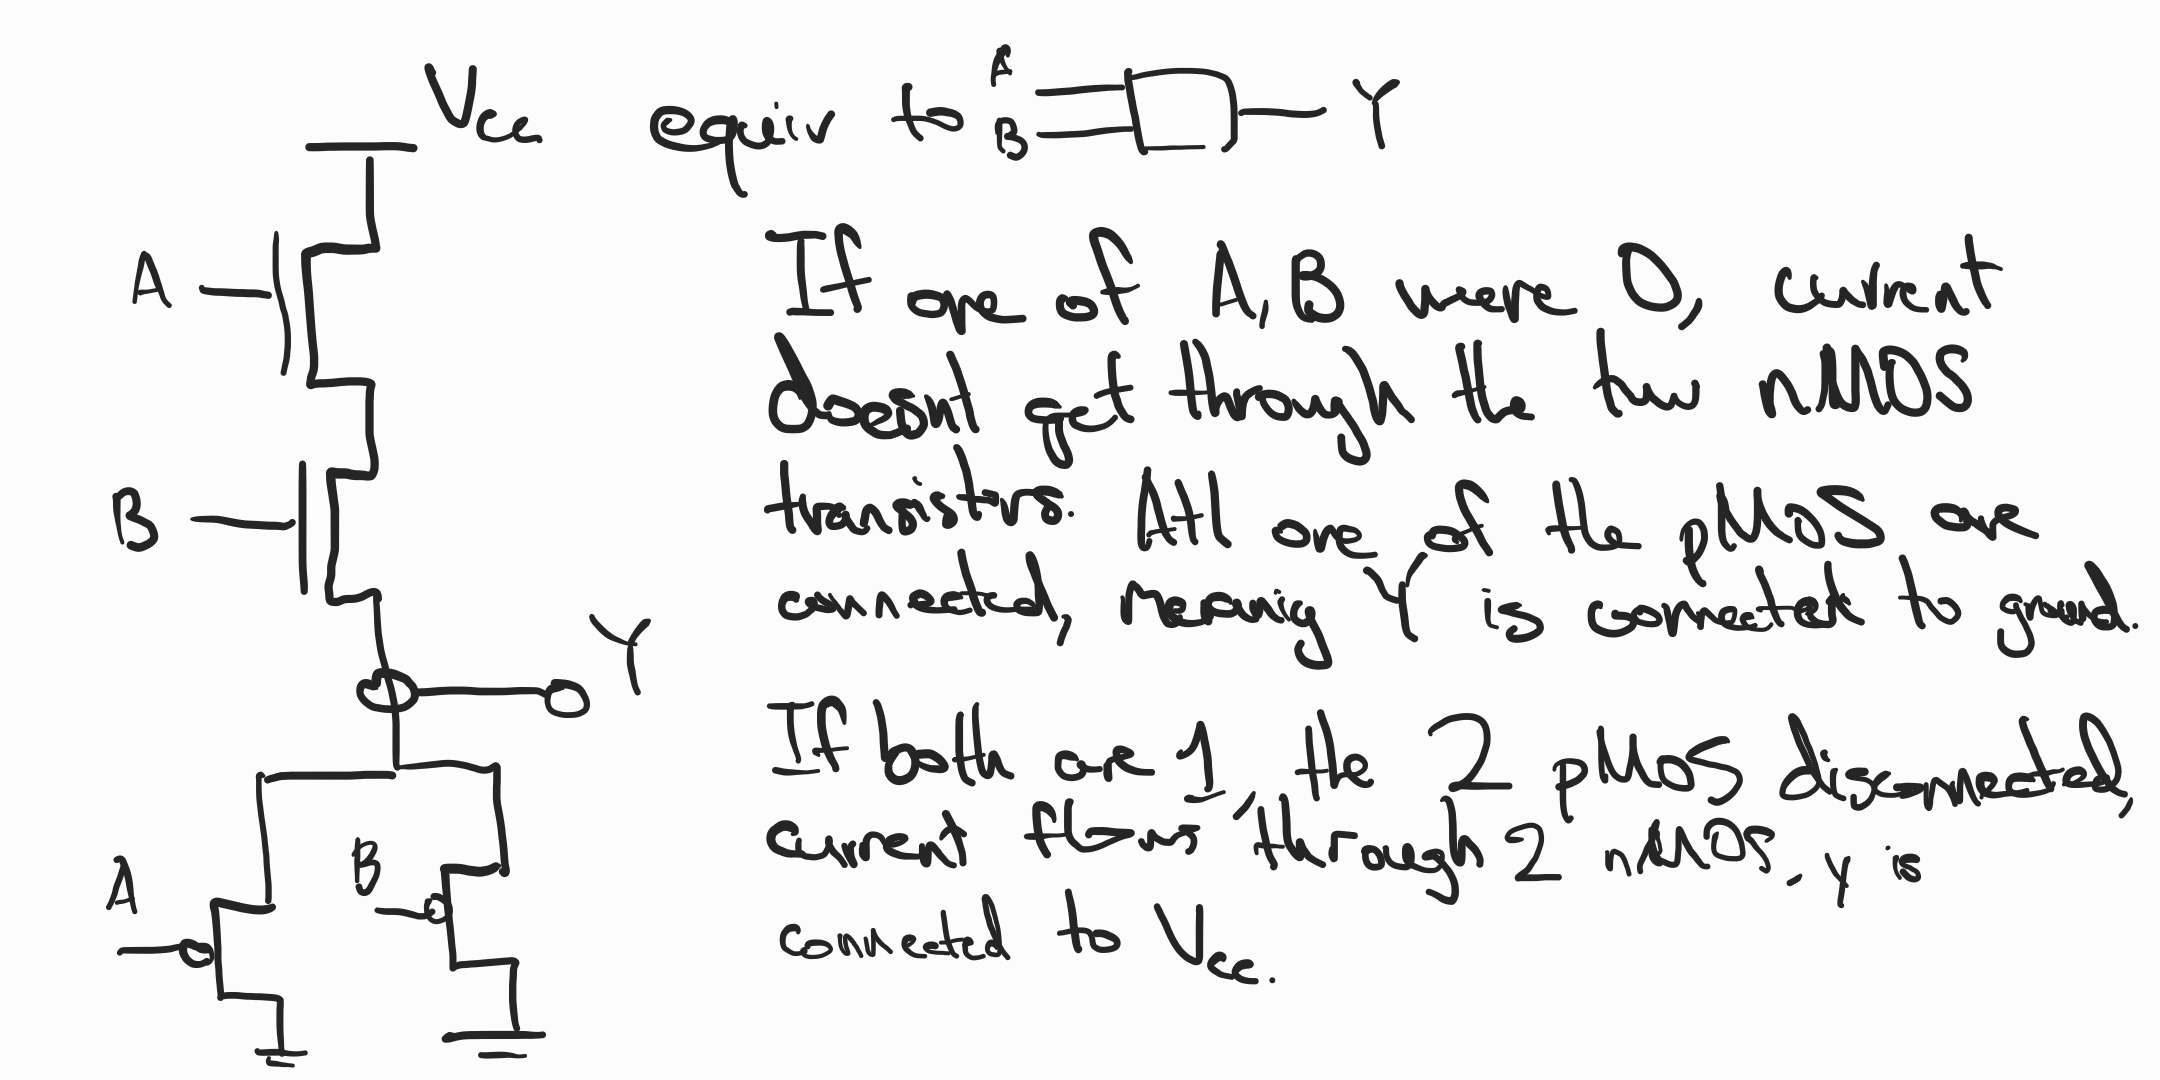
\includegraphics{csc258/figures/andgate.jpg}

We can build 3-input OR, AND gates and the like, but we will avoid making and using them in this course, as it's likely more convenient to use multiple OR and AND gates.

\subsection{Circuits}

Now that we understand how transistors and gates work, we wish them to use them to build circuits. In circuits, there is no need to worry about grounding and $V_{cc}$, the transistors take care of it for you, it's abstracted away.

\begin{problem}
    Given an input/output specification, we wish to connect circuit components to produce desired behavior. At the same time, we wish to save costs. \label{prob:nand}
\end{problem}

In lab 1 you will represent boolean expressions using logic gates. By convention AND takes precedence over OR. This means that $a \overline{b} + c$ actually means $(a \wedge \neg b) \vee c$. 

\subsubsection*{Circuit Creation and Minterms/Maxterms}

After this lecture, we should be able to build a truth table representing the desired behavior of the circuit you want to create, translate truth table rows into gates that implement said circuit, and finally use Karnaugh maps to reduce the circuit to the minimal number of gates.
\begin{enumerate}
    \item Produce a truth table (or use one that's given)
    \item Express truth table behavior as a boolean expression
    \item Convert this expression into gates
\end{enumerate}

Instead of repeatedly drawing NOT gates in this course, we say that $\neg A$ or $A'$ or $\overline{A}$ is the \textbf{complemented form} of $A$.

\begin{definition}[Minterm]
An AND expression with every input present in true or complemented form
\end{definition}
\begin{definition}[Maxterm]
An OR expression with every input present in true or complemented form.
\end{definition}

Given $n$ variables, to be a minterm/maxterm, all $n$ variables must be used. There exist exactly $2^n$ minterms and maxterms. Minterms and maxterms are also the \textbf{dual} of each other.\footnote{reminds me of disjunctive and conjunctive normal forms}

\begin{example}[Minterms and Maxterms]
    \textbf{Minterm}: $A \cdot \overline{B} \cdot C \cdot D$ \\ 
    \textbf{Maxterm}: $A + \overline{B} + C + \overline{D}$
\end{example}

In a truth table, a row corresponds to both a minterm $m_i$ and a maxterm $M_i$. In this course we mainly care about minterms, but maxterms are also testable. $m_i$ corresponds to the row in \textit{binary}. $m_{15}$ would describe the case where the output is low at all times except when $A = B = C = D = 1$. Maxterms are capitalized, such as $M_0 = A+B+C+D$, which is always high except for the case where all four input values are low.

If row $i$ corresponds to 1, then the minterm $m_i$ should evaluate to 1, consisting of the product of all variables $A_i$, with $A_i$ negated if the input is 0 for that row. If row $i$ corresponds to 0, then the maxterm $M_i$ should evaluate to 0, with the sum of all variables $\overline{A_i}$, with a variable not being negated when the input for it in that column is 0. 

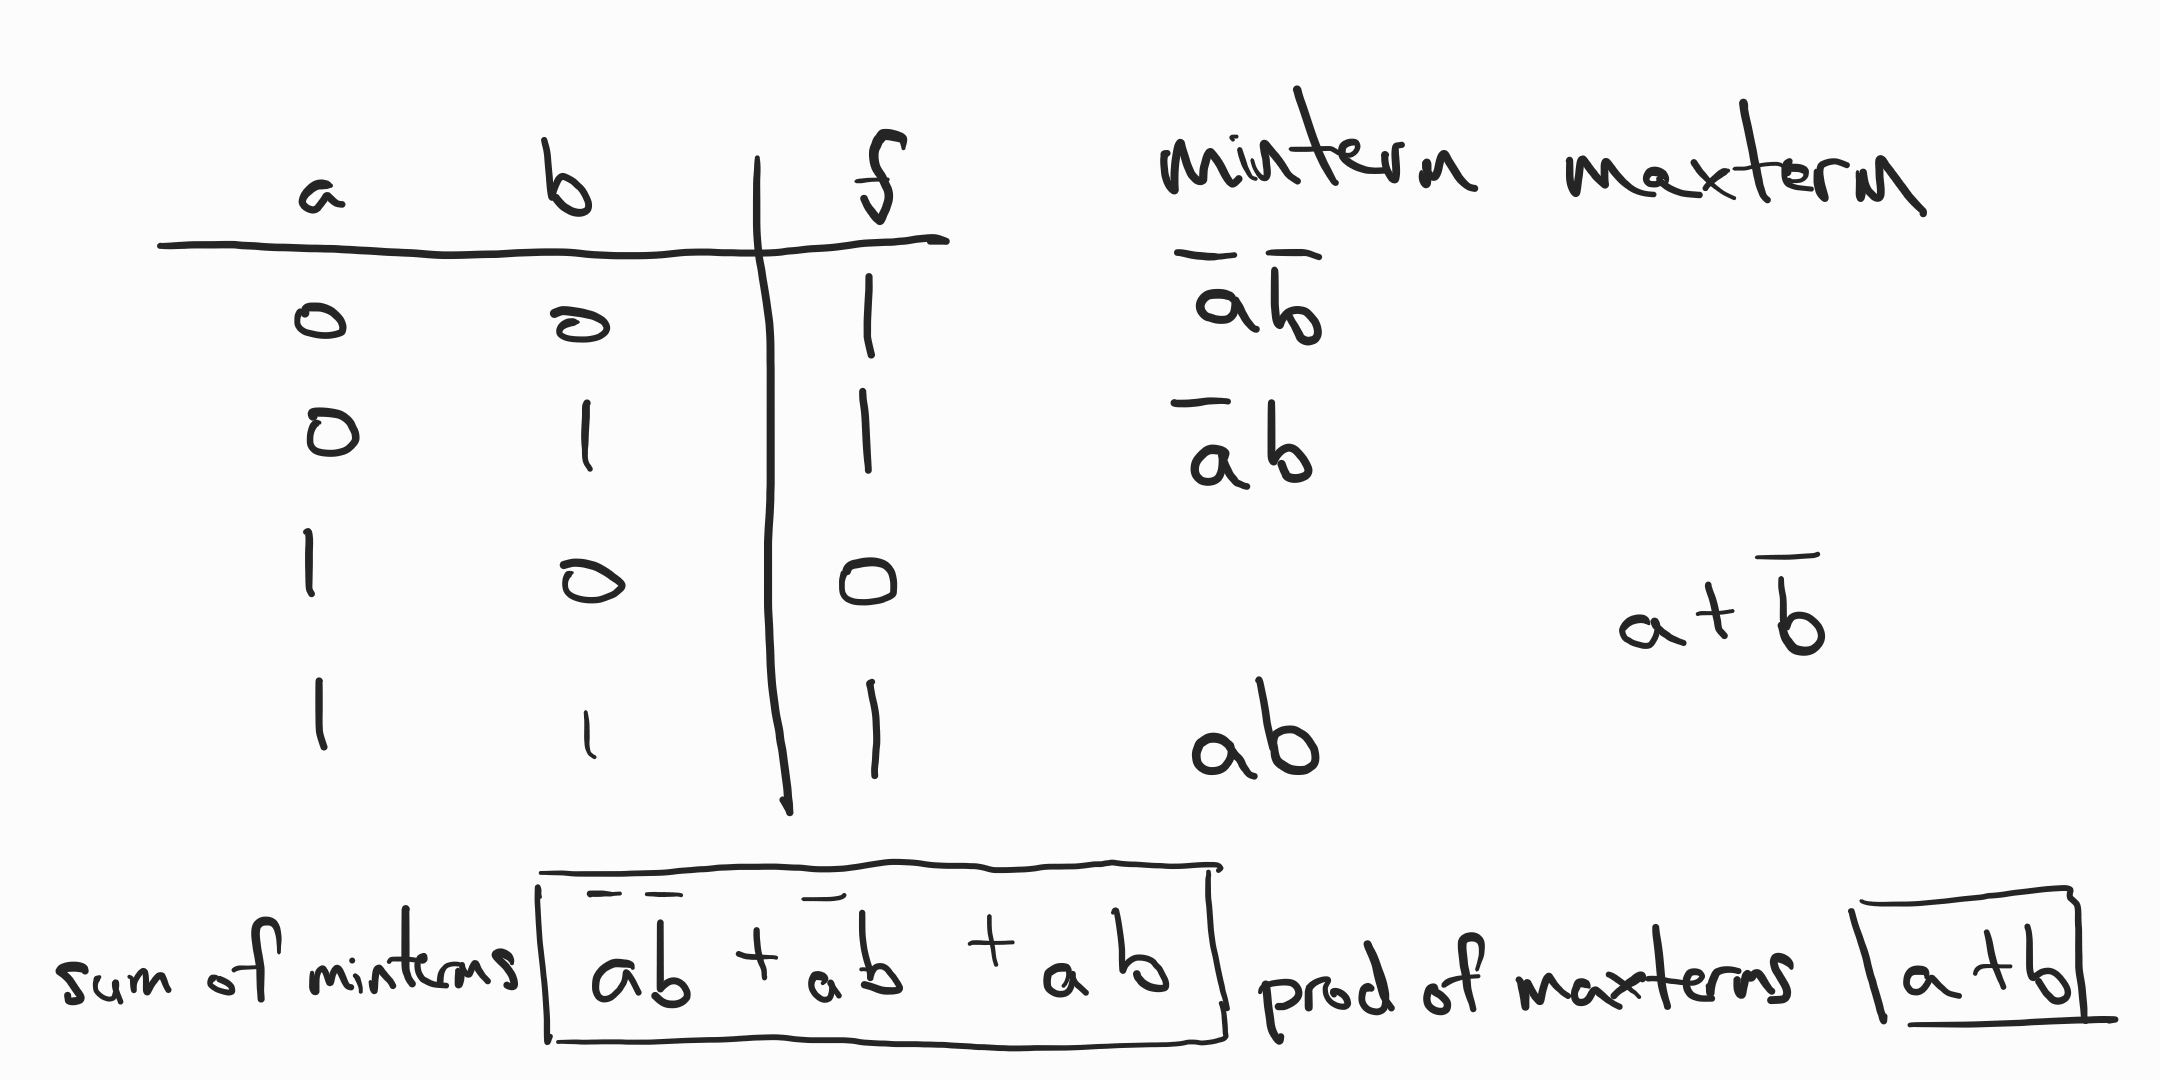
\includegraphics{csc258/figures/mintermmaxterm.jpg}

The goal is to join minterms and maxterms together to capture the truth table. The purpose of a minterm is to be true ONLY for that specific combination of input values. For a maxterm, it is to be false ONLY for that combination of input values. We can take sums (disjunctions) of minterms, to ensure that the expression is true iff it corresponds to a combination that makes it true. Can also take products (conjunctions) of maxterms, so that the expression is true iff everything is true, meaning the input values don't correspond to a false value. Both describe correct behavior.\footnote{would clean this explanation up}


\subsection{Back to Gates}

Once we have a sum-of-minterms expression, we can easily convert it to the equivalent combination of gates. Using DeMorgan's laws, we can convert everything to NAND gates, which are the cheapest to manufacture. Prof left proof as an exercise, which would solve problem \ref{prob:nand}.

To quantify how `simple' an expression is, we look at the \textbf{gate cost} (G) or the \textbf{gate cost with NOTs} (GN). To make something simpler, we attempt to combine terms.

A tool to derive the \textit{simplest possible circuit} is called the \textbf{Karnaugh map}. It's not always clear from looking at the truth table immediately, to draw a conclusion about which rows can be combined and simplified. Instead we can use a K-map to represent the same information, in a format that is easier to digest.

\begin{definition}[Karnaugh Map]
    K-maps are a grid of minterms/maxterms, arranged such that adjacent column/row labels in the grid differ by a single literal.\footnote{Rows and columns are ordered by Gray code instead of the usual binary, because this ordering has desirable properties.}
\end{definition}

\noindent With K-maps we wish to contain the 1s in boxes, satisfying some rules:
\begin{itemize}
\item Boxes must be rectangular, aligned with the map
\item Number of values contained within each box must be a power of 2
\item Boxes may overlap with each other
\item Boxes may wrap around the edges of the map
\end{itemize}

You can also use K-maps for max-terms, where you group zeroes together instead. There are theorems that show that the order of choosing the row and column labels of the K-map doesn't affect the final result, but the prof decided not to show them in class.
